\section{Collie River Basin 1 (model ID: 01)}
The Collie River Basin 1 model (fig.~\ref{fig:01_schematic}) is part of a top-down modelling exercise and is originally applied at the annual scale \citep{Jothityangkoon2001}. This is a classic bucket model. It has 1 store and 1 parameter ($S_{max}$). The model aims to represent:

\begin{itemizecompact}
\item Evaporation from soil moisture;
\item Saturation excess surface runoff.
\end{itemizecompact}

\subsection{MARRMoT model name}
m\_01\_collie1\_1p\_1s \\

% Equations
\subsection{Model equations}

% Model layout figure
{ 																	% This ensures it doesn't warp text further down
\begin{wrapfigure}{l}{4.5cm}
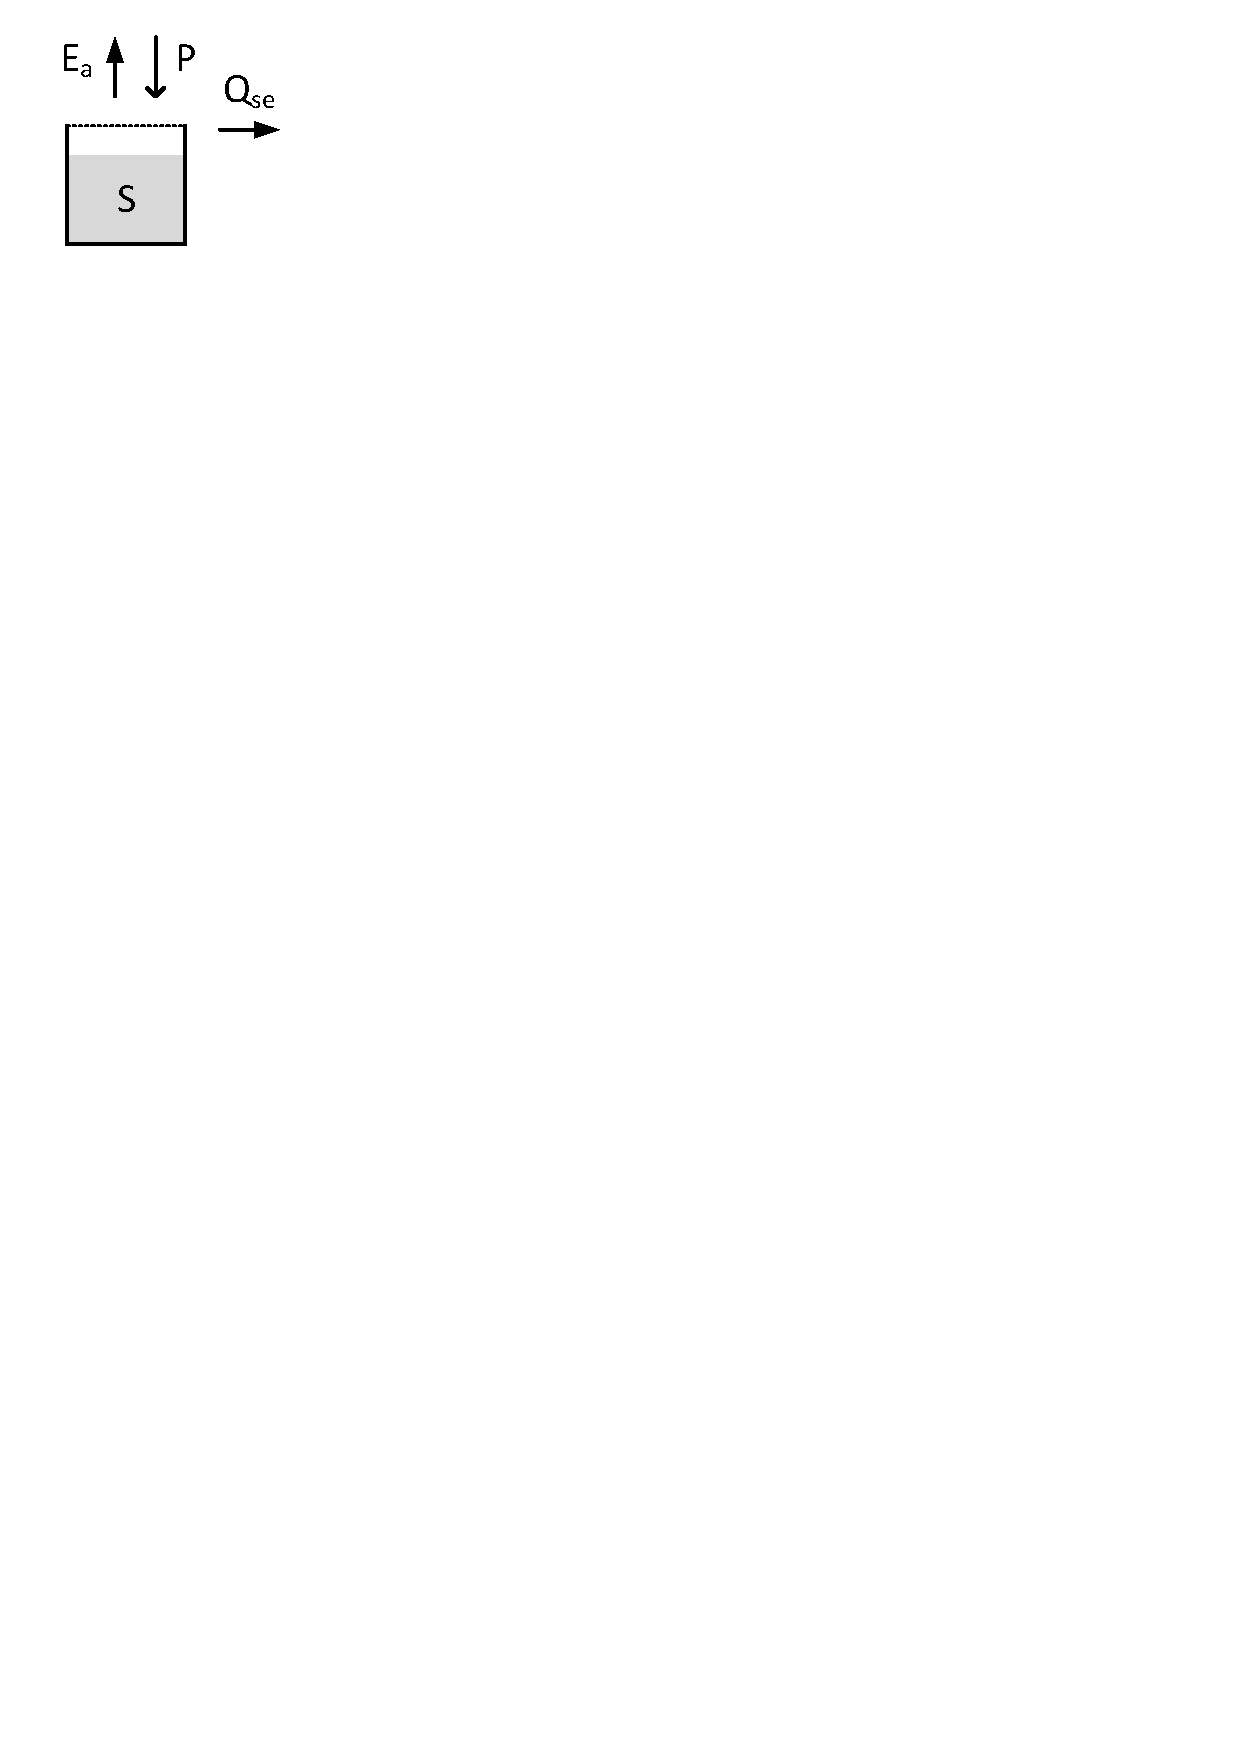
\includegraphics[trim=1cm 25.5cm 9cm 1cm,keepaspectratio]{./AppA_files/01_schematic.pdf}
\caption{Structure of the Collie River Basin 1 model} \label{fig:01_schematic}
\end{wrapfigure}

\begin{align}
	\frac{dS}{dt} &= P -E_a-Q_{se} \\
	Ea &= \frac{S}{S_{max}}*Ep\\
	Q_{se} &= 
		\begin{cases}
			P, & if~S>S_{max}\\
			0, & otherwise
		\end{cases}
\end{align}
}
\vspace{1.5cm}

Where  $S$ [mm] is the current storage in the soil moisture and $P$ the precipitation input $[mm/d]$. Actual evaporation $E_a$ $[mm/d]$ is estimated based on the current storage $S$, the maximum soil moisture storage $S_{max}$ [mm], and the potential evapotranspiration $E_p$ $[mm/d]$. $Q_{se}$ $[mm/d]$ is saturation excess overland flow.

\subsection{Parameter overview}
% Table generated by Excel2LaTeX from sheet 'Sheet1'
\begin{table}[htbp]
\centering
    \begin{tabular}{lll}
    \toprule
    Parameter & Unit  & Description \\
    \midrule
    $S_{max}$ & $mm$  & Maximum soil moisture storage \\
    \bottomrule
    \end{tabular}%
  \label{tab:addlabel}%
\end{table}%


